\documentclass[aspectratio=169]{beamer}
\usepackage{fontspec}
\usepackage{unicode-math}
\usepackage{tikz}
\usepackage{colortbl}
\usepackage{amsmath}
\usepackage{amssymb}
\usepackage{graphicx}
\usepackage{hyperref}
\usepackage{booktabs}
\usepackage{multirow}
\usepackage{xcolor}
\usepackage{listings}
\usepackage[style=apa,backend=biber,block=ragged,defernumbers=false]{biblatex}
\usepackage[linesnumbered,ruled,vlined]{algorithm2e}

% TikZ libraries
\usetikzlibrary{arrows,automata,positioning,shapes,calc,decorations.pathmorphing,patterns,math}

% Beamer theme
\usetheme{metropolis}

% Title page info
\title{Probabilistic Algorithms: What, Why, and How}
\subtitle{A Deep Dive into Randomness in Computing}
\author{Sailesh Dahal}
\institute{Kathmandu University}
\date{\today}

% Bibliography
\addbibresource{refs.bib}

% Listings configuration
\lstset{
    language=Python,
    basicstyle=\ttfamily\small,
    breaklines=true,
    frame=single,
    numbers=left,
    numberstyle=\tiny,
    keywordstyle=\color{blue},
    commentstyle=\color{green!60!black},
    stringstyle=\color{red},
    showstringspaces=false
}


\begin{document}

\begin{frame}
  \begin{tikzpicture}[remember picture,overlay]
    \node[anchor=south east, xshift=-5mm, yshift=5mm] at (current page.south east) {
      
\includegraphics[width=2cm]{./assets/ku_logo.png}
    };
  \end{tikzpicture}
  \titlepage
\end{frame}

% Outline frame
\begin{frame}{Outline}
  \tableofcontents
\end{frame}

% What are Probabilistic Algorithms?
\section{What are Probabilistic Algorithms?}
\begin{frame}{What is a Probabilistic Algorithm?}
  \begin{block}{Definition}
    An algorithm that makes random choices during execution to influence its behavior or output.
  \end{block}
\end{frame}

% Combined Visual: Deterministic vs Probabilistic Algorithm
\begin{frame}{Deterministic vs Probabilistic Algorithm}
  % Deterministic Algorithm (top)
  \begin{center}
    \begin{tikzpicture}
      % Box
      \node[draw, fill=yellow!80, minimum width=4cm, minimum height=1.5cm] (box) {\footnotesize Deterministic Algorithm};
      % Input arrow
      \node[left=1.5cm of box, align=center] (input) {\footnotesize Input $x$};
      \draw[->, thick] (input) -- (box);
      % Output arrow
      \node[right=1.5cm of box, align=center] (output) {\footnotesize Output $y$};
      \draw[->, thick] (box) -- (output);
    \end{tikzpicture}
    \\[0.2em]
    {\footnotesize Deterministic}
  \end{center}
  \vspace{1.5em}
  % Probabilistic Algorithm (bottom)
  \begin{center}
    \begin{tikzpicture}
      % Box
      \node[draw, fill=gray!30, minimum width=4cm, minimum height=1.5cm] (box) {\footnotesize Randomized Algorithm};
      % Input arrow
      \node[left=1.5cm of box, align=center] (input) {\footnotesize Input $x$};
      \draw[->, thick] (input) -- (box);
      % Output arrow
      \node[right=1.5cm of box, align=center] (output) {\footnotesize Output $y_r$};
      \draw[->, thick] (box) -- (output);
      % Random bits arrow
      \node[above=0.8cm of box, align=center] (rand) {\footnotesize random bits $r$};
      \draw[->, thick] (rand) -- (box);
    \end{tikzpicture}
    \\[0.2em]
    {\footnotesize Probabilistic}
  \end{center}
\end{frame}

\begin{frame}{Types of Probabilistic Algorithms}
  \begin{itemize}
    \item Las Vegas Algorithms \parencite{lasvegas1979babai}
    \item Monte Carlo Algorithms \parencite{Metropolis01091949}
  \end{itemize}
\end{frame}
% Expanded: Las Vegas Algorithms

\begin{frame}{Las Vegas Algorithms}
  \textbf{Definition:} A Las Vegas algorithm always produces a correct result or reports failure, with the running time depending on random choices. \parencite{LasVegasGupta1992}
\end{frame}

% Expanded: Monte Carlo Algorithms
\begin{frame}{Monte Carlo Algorithms}
  \textbf{Definition:} A Monte Carlo algorithm has a probability of producing an incorrect result, but its running time is bounded. \parencite{MonteCarloError1991}
\end{frame}

% New section for applications
\section{Applications of Probabilistic Algorithms}

\begin{frame}{Real-World Motivation}
  \begin{itemize}
    \item Web search (PageRank)
    \item Load balancing (power of two choices)
    \item Hashing (universal hash functions)
    \item Primality testing (Miller-Rabin)
  \end{itemize}
\end{frame}

% Why use Probabilistic Algorithms?
\section{Why Probabilistic Algorithms?}
\begin{frame}{Why Randomness?}
  \begin{block}{Motivation}
    \begin{itemize}
      \item Simpler algorithms

      \item Better expected performance

      \item Avoid worst-case scenarios

      \item Useful for large-scale and distributed systems
    \end{itemize}
  \end{block}
\end{frame}

% How do Probabilistic Algorithms work?
\section{How do Probabilistic Algorithms Work?}
\begin{frame}{How: Randomization in Algorithms}
  \begin{block}{Key Idea}
    Use random choices to influence the algorithm's path or output.
  \end{block}

  \begin{itemize}
    \item Random pivot in Quicksort

    \item Random walks in graphs

    \item Random sampling
  \end{itemize}
\end{frame}



\section{Example: Randomized Quicksort}

% New slide: QuickSort vs Randomized QuickSort steps
\begin{frame}{QuickSort vs Randomized QuickSort}
  \textbf{QuickSort:}
  \begin{enumerate}
    \item Pick a pivot element from the array \parencite{10.1093/comjnl/5.1.10}
    \item Split array into 3 subarrays: those smaller than pivot, those larger than pivot, and the pivot itself
    \item Recursively sort the subarrays, and concatenate them
  \end{enumerate}
  \vspace{1em}
  \textbf{Randomized QuickSort:}
  \begin{enumerate}
    \item Pick a pivot element \textbf{uniformly at random} from the array \parencite{motwani1995randomized}
    \item Split array into 3 subarrays: those smaller than pivot, those larger than pivot, and the pivot itself
    \item Recursively sort the subarrays, and concatenate them
  \end{enumerate}
\end{frame}

% New slide: Worst-case for QuickSort
\begin{frame}{Example: Randomized Quicksort}
  \textbf{Recall:} QuickSort can take $\Omega(n^2)$ time to sort an array of size $n$ \parencite{359631}
\end{frame}

% New slide: Theorem and expectation for Randomized QuickSort
\begin{frame}{Randomized QuickSort: Expected Runtime}
  \textbf{Theorem}
  \begin{block}{}
    Randomized QuickSort sorts a given array of length $n$ in $O(n \log n)$ expected time. \parencite{journals/acta/Sedgewick77}
  \end{block}
  \vspace{1em}
  \textbf{Note:} On every input, randomized QuickSort takes $O(n \log n)$ time in expectation. On every input, it may take $\Omega(n^2)$ time with some small probability.
\end{frame}

\subsection{Step-by-Step Execution}
\begin{frame}{Randomized Quicksort: Step 1 (Initial Array)}
  % Use columns for top-aligned split layout
  \begin{columns}[t]
    \column{0.6\textwidth}
    Consider the array:
    \[
      \renewcommand{\arraystretch}{1.5}
      \begin{array}{|c|c|c|c|c|c|c|c|}
        \hline
        15 & 3 & 1 & 10 & 9 & 0 & 6 & 4 \\
        \hline
      \end{array}
    \]
  \end{columns}
\end{frame}

\begin{frame}{Randomized Quicksort: Step 1.1 (Pivot Chosen)}
  % Use columns for top-aligned split layout
  \begin{columns}[t]
    \column{0.6\textwidth}
    Suppose the random pivot chosen is \textcolor{red}{10} (at index 3):
    \[
      \renewcommand{\arraystretch}{1.5}
      \begin{array}{|c|c|c|c|c|c|c|c|}
        \hline
        15 & 3 & 1 & \cellcolor{red!20}\textcolor{red}{10} & 9 & 0 & 6 & 4 \\
        \hline
      \end{array}
    \]
    \pause
    \column{0.38\textwidth}
    \begin{minipage}[t]{\linewidth}
      \vspace{0pt}
      \begin{center}
        \begin{tikzpicture}[
          scale=0.85,
          transform shape,
          level distance=1.5cm,
          level 1/.style={sibling distance=3.0cm},
          level 2/.style={sibling distance=2.0cm},
          level 3/.style={sibling distance=1.2cm},
          every node/.style={font=\tiny}
        ]
          \node[circle, draw, fill=green!20, minimum size=1cm, align=center] (root) {
            \textbf{A[0,7]} \\
            10
          };
        \end{tikzpicture}
      \end{center}
    \end{minipage}
  \end{columns}
\end{frame}
% Step 2: Partitioning around 10
\begin{frame}{Randomized Quicksort: Step 2 (Partitioning Around Pivot 10)}
  % Use columns for top-aligned split layout
  \begin{columns}[t]
    \column{0.6\textwidth}
    After selecting pivot 10, we partition the array:
    \begin{itemize}
      \item \textcolor{green!60!black}{Left:} 4, 3, 1, 9, 0, 6 (elements before pivot position)
      \item \textcolor{red}{Middle:} 10 (pivot)
      \item \textcolor{blue}{Right:} 15 (element after pivot position)
    \end{itemize}
    \pause
    After partitioning:
    \[
      \renewcommand{\arraystretch}{1.5}
      \begin{array}{|c|c|c|c|c|c|c|c|}
        \hline
        \cellcolor{green!20}\textcolor{green!60!black}{4} & \cellcolor{green!20}\textcolor{green!60!black}{3} & \cellcolor{green!20}\textcolor{green!60!black}{1} & \cellcolor{green!20}\textcolor{green!60!black}{9} & \cellcolor{green!20}\textcolor{green!60!black}{0} & \cellcolor{green!20}\textcolor{green!60!black}{6} & \cellcolor{red!20}\textcolor{red}{10} & 15 \\
        \hline
      \end{array}
    \]
    \pause
    \column{0.38\textwidth}
    \begin{minipage}[t]{\linewidth}
      \vspace{0pt}
      \begin{center}
        \begin{tikzpicture}[
          scale=0.85,
          transform shape,
          level distance=1.5cm,
          level 1/.style={sibling distance=3.0cm},
          level 2/.style={sibling distance=2.0cm},
          level 3/.style={sibling distance=1.2cm},
          every node/.style={font=\tiny}
        ]
          % Root node
          \node[circle, draw, fill=green!20, minimum size=1cm, align=center] (root) {
            \textbf{A[0,7]} \\
            10
          }
          % Left child
          child {node[circle, draw, fill=green!20, minimum size=1cm, align=center] {
                  \textbf{A[0,5]}
                }}
          % Right child
          child {node[circle, draw, fill=white, minimum size=1cm, align=center] {
                  \textbf{A[7,7]}
                }};
        \end{tikzpicture}
      \end{center}
    \end{minipage}
  \end{columns}
\end{frame}

% Step 3: Recurse Left [A[0,5]], Pivot 4
\begin{frame}{Randomized Quicksort: Step 3 (Recurse Left [A[0,5]], Pivot 4)}
  % Use columns for top-aligned split layout
  \begin{columns}[t]
    \column{0.6\textwidth}
    Recurse on the left subarray:
    \\[0.5em]
    Let's choose a random pivot, say 4.
    \[
      \renewcommand{\arraystretch}{1.5}
      \begin{array}{|c|c|c|c|c|c|}
        \hline
        \cellcolor{red!20}\textcolor{red}{4} & 3 & 1 & 9 & 0 & 6 \\
        \hline
      \end{array}
    \]
    \pause
    \column{0.38\textwidth}
    \begin{minipage}[t]{\linewidth}
      \vspace{0pt}
      \begin{center}
        \begin{tikzpicture}[
          scale=0.85,
          transform shape,
          level distance=1.5cm,
          level 1/.style={sibling distance=3.0cm},
          level 2/.style={sibling distance=2.0cm},
          level 3/.style={sibling distance=1.2cm},
          every node/.style={font=\tiny}
        ]
          % Root node
          \node[circle, draw, fill=green!20, minimum size=1cm, align=center] (root) {
            \textbf{A[0,7]} \\
            10
          }
          % Left child
          child {node[circle, draw, fill=green!20, minimum size=1cm, align=center] {
                  \textbf{A[0,5]} \\
                  4
                }}
          % Right child
          child {node[circle, draw, fill=white, minimum size=1cm, align=center] {
                  \textbf{A[7,7]}
                }};
        \end{tikzpicture}
      \end{center}
    \end{minipage}
  \end{columns}
\end{frame}

% Step 3.1: Partition Left [A[0,5]] Around 4
\begin{frame}{Randomized Quicksort: Step 3.1 (Partition Left [A[0,5]] Around 4)}
  % Use columns for top-aligned split layout
  \begin{columns}[t]
    \column{0.6\textwidth}
    After partitioning the left subarray:
    \[
      \renewcommand{\arraystretch}{1.5}
      \begin{array}{|c|c|c|c|c|c|}
        \hline
        \cellcolor{green!20}\textcolor{green!60!black}{0} & \cellcolor{green!20}\textcolor{green!60!black}{3} & \cellcolor{green!20}\textcolor{green!60!black}{1} & \cellcolor{red!20}\textcolor{red}{4} & 9 & 6 \\
        \hline
      \end{array}
    \]
    Partition:
    \begin{itemize}
      \item \textcolor{green!60!black}{Left:} 0, 3, 1 (elements before pivot)
      \item \textcolor{red}{Middle:} 4 (pivot)
      \item \textcolor{blue}{Right:} 9, 6 (elements after pivot)
    \end{itemize}
    \pause
    \column{0.38\textwidth}
    \begin{minipage}[t]{\linewidth}
      \vspace{0pt}
      \begin{center}
        \begin{tikzpicture}[
          scale=0.85,
          transform shape,
          level distance=1.5cm,
          level 1/.style={sibling distance=3.0cm},
          level 2/.style={sibling distance=2.0cm},
          level 3/.style={sibling distance=1.2cm},
          every node/.style={font=\tiny}
        ]
          % Root node
          \node[circle, draw, fill=green!20, minimum size=1cm, align=center] (root) {
            \textbf{A[0,7]} \\
            10
          }
          % Left child
          child {node[circle, draw, fill=green!20, minimum size=1cm, align=center] {
                  \textbf{A[0,5]} \\
                  4
                }
              child {node[circle, draw, fill=white, minimum size=1cm, align=center] {
                      \textbf{A[0,2]}
                    }}
              child {node[circle, draw, fill=white, minimum size=1cm, align=center] {
                      \textbf{A[4,5]}
                    }}
            }
          % Right child
          child {node[circle, draw, fill=white, minimum size=1cm, align=center] {
                  \textbf{A[7,7]}
                }};
        \end{tikzpicture}
      \end{center}
    \end{minipage}
  \end{columns}
\end{frame}

% Step 3.1.1: Recurse Left [A[0,2]], Pivot 0
\begin{frame}{Randomized Quicksort: Step 3.1.1 (Recurse Left [A[0,2]], Pivot 0)}
  % Use columns for top-aligned split layout
  \begin{columns}[t]
    \column{0.6\textwidth}
    Recurse on the left subarray:
    \\[0.5em]
    Let's choose a random pivot, say 0.
    \[
      \renewcommand{\arraystretch}{1.5}
      \begin{array}{|c|c|c|}
        \hline
        \cellcolor{red!20}\textcolor{red}{0} & 3 & 1 \\
        \hline
      \end{array}
    \]
    \pause
    \column{0.38\textwidth}
    \begin{minipage}[t]{\linewidth}
      \vspace{0pt}
      \begin{center}
        \begin{tikzpicture}[
          scale=0.85,
          transform shape,
          level distance=1.5cm,
          level 1/.style={sibling distance=3.0cm},
          level 2/.style={sibling distance=2.0cm},
          level 3/.style={sibling distance=1.2cm},
          every node/.style={font=\tiny}
        ]
          % Root node
          \node[circle, draw, fill=green!20, minimum size=1cm, align=center] (root) {
            \textbf{A[0,7]} \\
            10
          }
          % Left child
          child {node[circle, draw, fill=green!20, minimum size=1cm, align=center] {
                  \textbf{A[0,5]} \\
                  4
                }
              child {node[circle, draw, fill=green!20, minimum size=1cm, align=center] {
                      \textbf{A[0,2]}\\
                      0
                    }}
              child {node[circle, draw, fill=white, minimum size=1cm, align=center] {
                      \textbf{A[4,5]}
                    }}
            }
          % Right child
          child {node[circle, draw, fill=white, minimum size=1cm, align=center] {
                  \textbf{A[7,7]}
                }
            };
        \end{tikzpicture}
      \end{center}
    \end{minipage}
  \end{columns}
\end{frame}

% Step 3.1.1.1: Partition Left [A[0,2]] Around 0
\begin{frame}{Randomized Quicksort: Step 3.1.1.1 (Partition Left [A[0,2]] Around 0)}
  % Use columns for top-aligned split layout
  \begin{columns}[t]
    \column{0.6\textwidth}
    After partitioning the left subarray:
    \[
      \renewcommand{\arraystretch}{1.5}
      \begin{array}{|c|c|c|}
        \hline
        \cellcolor{red!20}\textcolor{red}{0} & 3 & 1 \\
        \hline
      \end{array}
    \]
    Partition:
    \begin{itemize}
      \item \textcolor{green!60!black}{Left:} (empty)
      \item \textcolor{red}{Middle:} 0 (pivot)
      \item \textcolor{blue}{Right:} 3, 1 (elements after pivot)
    \end{itemize}
    \pause
    \column{0.38\textwidth}
    \begin{minipage}[t]{\linewidth}
      \vspace{0pt}
      \begin{center}
        \begin{tikzpicture}[
          scale=0.85,
          transform shape,
          level distance=1.5cm,
          level 1/.style={sibling distance=3.0cm},
          level 2/.style={sibling distance=2.0cm},
          level 3/.style={sibling distance=1.2cm},
          every node/.style={font=\tiny}
        ]
          % Root node
          \node[circle, draw, fill=green!20, minimum size=1cm, align=center] (root) {
            \textbf{A[0,7]} \\
            10
          }
          % Left child
          child {node[circle, draw, fill=green!20, minimum size=1cm, align=center] {
                  \textbf{A[0,5]} \\
                  4
                }
              child {node[circle, draw, fill=green!20, minimum size=1cm, align=center] {
                      \textbf{A[0,2]}\\
                      0
                    }
                  child {node[circle, draw, fill=red!40, minimum size=1cm, align=center] {
                          \textbf{A[0,-1]}
                        }}
                  child {node[circle, draw, fill=white, minimum size=1cm, align=center] {
                          \textbf{A[1,2]}
                        }}
                }
              child {node[circle, draw, fill=white, minimum size=1cm, align=center] {
                      \textbf{A[4,5]}
                    }}
            }
          % Right child
          child {node[circle, draw, fill=white, minimum size=1cm, align=center] {
                  \textbf{A[7,7]}
                }
            };
        \end{tikzpicture}
      \end{center}
    \end{minipage}
  \end{columns}
\end{frame}

\begin{frame}{Randomized Quicksort: Step 3.1.1.2 (Recurse Right [A[1,2]], Pivot 3)}
  % Use columns for top-aligned split layout
  \begin{columns}[t]
    \column{0.6\textwidth}
    Recurse on the right subarray:
    \\[0.5em]
    Let's choose a random pivot, say 3.
    \[
      \renewcommand{\arraystretch}{1.5}
      \begin{array}{|c|c|}
        \hline
        \cellcolor{red!20}\textcolor{red}{3} & 1 \\
        \hline
      \end{array}
    \]
    \pause
    \column{0.38\textwidth}
    \begin{minipage}[t]{\linewidth}
      \vspace{0pt}
      \begin{center}
        \begin{tikzpicture}[
          scale=0.85,
          transform shape,
          level distance=1.5cm,
          level 1/.style={sibling distance=3.0cm},
          level 2/.style={sibling distance=2.0cm},
          level 3/.style={sibling distance=1.2cm},
          every node/.style={font=\tiny}
        ]
          % Root node
          \node[circle, draw, fill=green!20, minimum size=1cm, align=center] (root) {
            \textbf{A[0,7]} \\
            10
          }
          % Left child
          child {node[circle, draw, fill=green!20, minimum size=1cm, align=center] {
                  \textbf{A[0,5]} \\
                  4
                }
              child {node[circle, draw, fill=green!20, minimum size=1cm, align=center] {
                      \textbf{A[0,2]}\\
                      0
                    }
                  child {node[circle, draw, fill=red!40, minimum size=1cm, align=center] {
                          \textbf{A[0,-1]}
                        }}
                  child {node[circle, draw, fill=green!20, minimum size=1cm, align=center] {
                          \textbf{A[1,2]}\\
                          3
                        }
                    }
                }
              child {node[circle, draw, fill=white, minimum size=1cm, align=center] {
                      \textbf{A[4,5]}
                    }}
            }
          % Right child
          child {node[circle, draw, fill=white, minimum size=1cm, align=center] {
                  \textbf{A[7,7]}
                }
            };
        \end{tikzpicture}
      \end{center}
    \end{minipage}
  \end{columns}
\end{frame}

% Step 3.1.1.2.1: Partition [A[1,2]] Around 3
\begin{frame}{Randomized Quicksort: Step 3.1.1.2.1 (Partition [A[1,2]] Around 3)}
  % Use columns for top-aligned split layout
  \begin{columns}[t]
    \column{0.6\textwidth}
    After partitioning the left subarray:
    \[
      \renewcommand{\arraystretch}{1.5}
      \begin{array}{|c|c|c|}
        \hline
        1 & \cellcolor{red!20}\textcolor{red}{3} \\
        \hline
      \end{array}
    \]
    Partition:
    \begin{itemize}
      \item \textcolor{green!60!black}{Left:} 1 (element before pivot)
      \item \textcolor{red}{Middle:} 3 (pivot)
      \item \textcolor{blue}{Right:} (empty)
    \end{itemize}
    \pause
    \column{0.38\textwidth}
    \begin{minipage}[t]{\linewidth}
      \vspace{0pt} % Ensures true top alignment
      \begin{center}

        \begin{tikzpicture}[
          scale=0.85,
          transform shape,
          level distance=1.5cm,
          level 1/.style={sibling distance=3.0cm},
          level 2/.style={sibling distance=2.0cm},
          level 3/.style={sibling distance=1.2cm},
          every node/.style={font=\tiny}
        ]
          % Root node
          \node[circle, draw, fill=green!20, minimum size=1cm, align=center] (root) {
            \textbf{A[0,7]} \\
            10
          }
          % Left child
          child {node[circle, draw, fill=green!20, minimum size=1cm, align=center] {
                  \textbf{A[0,5]} \\
                  4
                }
              child {node[circle, draw, fill=green!20, minimum size=1cm, align=center] {
                      \textbf{A[0,2]}\\
                      0
                    }
                  child {node[circle, draw, fill=red!40, minimum size=1cm, align=center] {
                          \textbf{A[0,-1]}
                        }}
                  child {node[circle, draw, fill=green!20, minimum size=1cm, align=center] {
                          \textbf{A[1,2]}\\
                          3
                        }
                      child {node[circle, draw, fill=blue!20, minimum size=1cm, align=center] {
                              \textbf{A[1,1]}
                            }
                        }
                      child {node[circle, draw, fill=white, minimum size=1cm, align=center] {
                              \textbf{A[3,2]}
                            }
                        }
                    }
                }
              child {node[circle, draw, fill=white, minimum size=1cm, align=center] {
                      \textbf{A[4,5]}
                    }}
            }
          % Right child
          child {node[circle, draw, fill=white, minimum size=1cm, align=center] {
                  \textbf{A[7,7]}
                }
            };
        \end{tikzpicture}
      \end{center}
    \end{minipage}
  \end{columns}
\end{frame}

% Step 3.1.1.2.1.1: Recurse Left [A[1,1]], Done
\begin{frame}{Randomized Quicksort: Step 3.1.1.2.1.1 (Recurse Left [A[1,1]], Done)}
  \begin{columns}[t]
    \column{0.6\textwidth}
    After partitioning the left subarray:
    \[
      \renewcommand{\arraystretch}{1.5}
      \begin{array}{|c|c|c|}
        \hline
        \cellcolor{green!20}{1} \\
        \hline
      \end{array}
    \]

    Partition:
    \begin{itemize}
      \item \textcolor{green!60!black}{Left:} (empty)
      \item \textcolor{red}{Middle:} 1 (pivot)
      \item \textcolor{blue}{Right:} (empty)
    \end{itemize}
    Single element subarray, done, return.
    \column{0.38\textwidth}
    \begin{minipage}[t]{\linewidth}
      \vspace{0pt} % Ensures true top alignment
      \begin{center}

        \begin{tikzpicture}[
          scale=0.85,
          transform shape,
          level distance=1.5cm,
          level 1/.style={sibling distance=3.0cm},
          level 2/.style={sibling distance=2.0cm},
          level 3/.style={sibling distance=1.2cm},
          every node/.style={font=\tiny}
        ]
          % Root node
          \node[circle, draw, fill=green!20, minimum size=1cm, align=center] (root) {
            \textbf{A[0,7]} \\
            10
          }
          % Left child
          child {node[circle, draw, fill=green!20, minimum size=1cm, align=center] {
                  \textbf{A[0,5]} \\
                  4
                }
              child {node[circle, draw, fill=green!20, minimum size=1cm, align=center] {
                      \textbf{A[0,2]}\\
                      0
                    }
                  child {node[circle, draw, fill=red!40, minimum size=1cm, align=center] {
                          \textbf{A[0,-1]}
                        }}
                  child {node[circle, draw, fill=green!20, minimum size=1cm, align=center] {
                          \textbf{A[1,2]}\\
                          3
                        }
                      child {node[circle, draw, fill=blue!20, minimum size=1cm, align=center] {
                              \textbf{A[1,1]}
                            }
                        }
                      child {node[circle, draw, fill=red!40, minimum size=1cm, align=center] {
                              \textbf{A[3,2]}
                            }
                        }
                    }
                }
              child {node[circle, draw, fill=white, minimum size=1cm, align=center] {
                      \textbf{A[4,5]}
                    }}
            }
          % Right child
          child {node[circle, draw, fill=white, minimum size=1cm, align=center] {
                  \textbf{A[7,7]}
                }
            };
        \end{tikzpicture}
      \end{center}
    \end{minipage}
  \end{columns}
\end{frame}

% Step 3.1.1.2.1.2: Recurse Right [A[3,2]], Done
\begin{frame}{Randomized Quicksort: Step 3.1.1.2.1.2 (Recurse Right [A[3,2]], Done)}
  \begin{columns}[t]
    \column{0.6\textwidth}
    Recurse on the right subarray $A[3,2]$ (empty, done).
    Return to parent call $A[1,2]$
    \column{0.38\textwidth}
    \begin{minipage}[t]{\linewidth}
      \vspace{0pt} % Ensures true top alignment
      \begin{center}

        \begin{tikzpicture}[
          scale=0.85,
          transform shape,
          level distance=1.5cm,
          level 1/.style={sibling distance=3.0cm},
          level 2/.style={sibling distance=2.0cm},
          level 3/.style={sibling distance=1.2cm},
          every node/.style={font=\tiny}
        ]
          % Root node
          \node[circle, draw, fill=green!20, minimum size=1cm, align=center] (root) {
            \textbf{A[0,7]} \\
            10
          }
          % Left child
          child {node[circle, draw, fill=green!20, minimum size=1cm, align=center] {
                  \textbf{A[0,5]} \\
                  4
                }
              child {node[circle, draw, fill=green!20, minimum size=1cm, align=center] {
                      \textbf{A[0,2]}\\
                      0
                    }
                  child {node[circle, draw, fill=red!40, minimum size=1cm, align=center] {
                          \textbf{A[0,-1]}
                        }}
                  child {node[circle, draw, fill=green!20, minimum size=1cm, align=center] {
                          \textbf{A[1,2]}\\
                          3
                        }
                      child {node[circle, draw, fill=blue!20, minimum size=1cm, align=center] {
                              \textbf{A[1,1]}
                            }
                        }
                      child {node[circle, draw, fill=red!40, minimum size=1cm, align=center] {
                              \textbf{A[3,2]}
                            }
                        }
                    }
                }
              child {node[circle, draw, fill=white, minimum size=1cm, align=center] {
                      \textbf{A[4,5]}
                    }}
            }
          % Right child
          child {node[circle, draw, fill=white, minimum size=1cm, align=center] {
                  \textbf{A[7,7]}
                }
            };
        \end{tikzpicture}
      \end{center}
    \end{minipage}
  \end{columns}
\end{frame}

% Step 3.1.2: Return to [A[0,2]]
\begin{frame}{Randomized Quicksort: Step 3.1.2 (Return to [A[0,2]])}
  \begin{columns}[t]
    \column{0.6\textwidth}
    Return to parent call $A[0,2]$
    \column{0.38\textwidth}
    \begin{minipage}[t]{\linewidth}
      \vspace{0pt} % Ensures true top alignment
      \begin{center}

        \begin{tikzpicture}[
          scale=0.85,
          transform shape,
          level distance=1.5cm,
          level 1/.style={sibling distance=3.0cm},
          level 2/.style={sibling distance=2.0cm},
          level 3/.style={sibling distance=1.2cm},
          every node/.style={font=\tiny}
        ]
          % Root node
          \node[circle, draw, fill=green!20, minimum size=1cm, align=center] (root) {
            \textbf{A[0,7]} \\
            10
          }
          % Left child
          child {node[circle, draw, fill=green!20, minimum size=1cm, align=center] {
                  \textbf{A[0,5]} \\
                  4
                }
              child {node[circle, draw, fill=green!20, minimum size=1cm, align=center] {
                      \textbf{A[0,2]}\\
                      0
                    }
                  child {node[circle, draw, fill=red!40, minimum size=1cm, align=center] {
                          \textbf{A[0,-1]}
                        }}
                  child {node[circle, draw, fill=blue!20, minimum size=1cm, align=center] {
                          \textbf{A[1,2]}\\
                          3
                        }
                      child {node[circle, draw, fill=blue!20, minimum size=1cm, align=center] {
                              \textbf{A[1,1]}\\
                              1
                            }
                        }
                      child {node[circle, draw, fill=red!40, minimum size=1cm, align=center] {
                              \textbf{A[3,2]}
                            }
                        }
                    }
                }
              child {node[circle, draw, fill=white, minimum size=1cm, align=center] {
                      \textbf{A[4,5]}
                    }}
            }
          % Right child
          child {node[circle, draw, fill=white, minimum size=1cm, align=center] {
                  \textbf{A[7,7]}
                }
            };
        \end{tikzpicture}
      \end{center}
    \end{minipage}
  \end{columns}
\end{frame}

% Step 3.2: Recurse Right [A[4,5]], Pivot 9
\begin{frame}{Randomized Quicksort: Step 3.2 (Recurse Right [A[4,5]], Pivot 9)}
  \begin{columns}[t]
    \column{0.6\textwidth}
    Recurse on the right subarray $A[4,5]$:
    \\[0.5em]
    Let's choose a random pivot, say 9.
    \[
      \renewcommand{\arraystretch}{1.5}
      \begin{array}{|c|c|}
        \hline
        \cellcolor{red!20}\textcolor{red}{9} & 6 \\
        \hline
      \end{array}
    \]
    \pause
    \column{0.38\textwidth}
    \begin{minipage}[t]{\linewidth}
      \vspace{0pt} % Ensures true top alignment
      \begin{center}

        \begin{tikzpicture}[
          scale=0.85,
          transform shape,
          level distance=1.5cm,
          level 1/.style={sibling distance=3.0cm},
          level 2/.style={sibling distance=2.0cm},
          level 3/.style={sibling distance=1.2cm},
          every node/.style={font=\tiny}
        ]
          % Root node
          \node[circle, draw, fill=green!20, minimum size=1cm, align=center] (root) {
            \textbf{A[0,7]} \\
            10
          }
          % Left child
          child {node[circle, draw, fill=green!20, minimum size=1cm, align=center] {
                  \textbf{A[0,5]} \\
                  4
                }
              child {node[circle, draw, fill=green!20, minimum size=1cm, align=center] {
                      \textbf{A[0,2]}\\
                      0
                    }
                  child {node[circle, draw, fill=red!40, minimum size=1cm, align=center] {
                          \textbf{A[0,-1]}
                        }}
                  child {node[circle, draw, fill=blue!20, minimum size=1cm, align=center] {
                          \textbf{A[1,2]}\\
                          3
                        }
                      child {node[circle, draw, fill=blue!20, minimum size=1cm, align=center] {
                              \textbf{A[1,1]}\\
                              1
                            }
                        }
                      child {node[circle, draw, fill=red!40, minimum size=1cm, align=center] {
                              \textbf{A[3,2]}
                            }
                        }
                    }
                }
              child {node[circle, draw, fill=green!20, minimum size=1cm, align=center] {
                      \textbf{A[4,5]}\\
                      9
                    }
                    child {node[circle, draw, fill=white, minimum size=1cm, align=center] {
                    \textbf{A[4,4]}
                        }}
                  child {node[circle, draw, fill=white, minimum size=1cm, align=center] {
                      \textbf{A[6,5]}
                    }}
                  }
            }
          % Right child
          child {node[circle, draw, fill=white, minimum size=1cm, align=center] {
                  \textbf{A[7,7]}
                }
            };
        \end{tikzpicture}
      \end{center}
    \end{minipage}
  \end{columns}
\end{frame}

% Step 3.2.1: Partition [A[4,5]] Around 9
\begin{frame}{Randomized Quicksort: Step 3.2.1 (Partition [A[4,5]] Around 9)}
  \begin{columns}[t]
    \column{0.6\textwidth}
    Recurse on the right subarray $A[4,5]$:
    \\[0.5em]

    Suppose the random pivot is \textcolor{red}{9}:
    \[
      \renewcommand{\arraystretch}{1.5}
      \begin{array}{|c|c|}
        \hline
        6 & \cellcolor{red!20}\textcolor{red}{9} \\
        \hline
      \end{array}
    \]

    Partition:
    \begin{itemize}
      \item \textcolor{green!60!black}{Left:} 6 (element before pivot)
      \item \textcolor{red}{Middle:} 9 (pivot)
      \item \textcolor{blue}{Right:} (empty)
    \end{itemize}
    \pause
    \column{0.38\textwidth}
    \begin{minipage}[t]{\linewidth}
      \vspace{0pt} % Ensures true top alignment
      \begin{center}

        \begin{tikzpicture}[
          scale=0.85,
          transform shape,
          level distance=1.5cm,
          level 1/.style={sibling distance=3.0cm},
          level 2/.style={sibling distance=2.0cm},
          level 3/.style={sibling distance=1.2cm},
          every node/.style={font=\tiny}
        ]
          % Root node
          \node[circle, draw, fill=green!20, minimum size=1cm, align=center] (root) {
            \textbf{A[0,7]} \\
            10
          }
          % Left child
          child {node[circle, draw, fill=green!20, minimum size=1cm, align=center] {
                  \textbf{A[0,5]} \\
                  4
                }
              child {node[circle, draw, fill=green!20, minimum size=1cm, align=center] {
                      \textbf{A[0,2]}\\
                      0
                    }
                  child {node[circle, draw, fill=red!40, minimum size=1cm, align=center] {
                          \textbf{A[0,-1]}
                        }}
                  child {node[circle, draw, fill=blue!20, minimum size=1cm, align=center] {
                          \textbf{A[1,2]}\\
                          3
                        }
                      child {node[circle, draw, fill=blue!20, minimum size=1cm, align=center] {
                              \textbf{A[1,1]}\\
                              1
                            }
                        }
                      child {node[circle, draw, fill=red!40, minimum size=1cm, align=center] {
                              \textbf{A[3,2]}
                            }
                        }
                    }
                }
              child {node[circle, draw, fill=green!20, minimum size=1cm, align=center] {
                      \textbf{A[4,5]}\\
                      9
                    }
                  child {node[circle, draw, fill=white, minimum size=1cm, align=center] {
                          \textbf{A[4,4]}
                        }}
                  child {node[circle, draw, fill=white, minimum size=1cm, align=center] {
                          \textbf{A[6,5]}
                        }}
                }
            }
          % Right child
          child {node[circle, draw, fill=white, minimum size=1cm, align=center] {
                  \textbf{A[7,7]}
                }
            };
        \end{tikzpicture}
      \end{center}
    \end{minipage}
  \end{columns}
\end{frame}

% Step 3.2.1.1: Recurse Left [A[4,4]], Done
\begin{frame}{Randomized Quicksort: Step 3.2.1.1 (Recurse Left [A[4,4]], Done)}
  \begin{columns}[t]
    \column{0.6\textwidth}
    After partitioning the left subarray:
    \[
      \renewcommand{\arraystretch}{1.5}
      \begin{array}{|c|c|c|}
        \hline
        \cellcolor{green!20}{6} \\
        \hline
      \end{array}
    \]

    Partition:
    \begin{itemize}
      \item \textcolor{green!60!black}{Left:} (empty)
      \item \textcolor{red}{Middle:} 6 (pivot)
      \item \textcolor{blue}{Right:} (empty)
    \end{itemize}
    Single element subarray, done, return.
    \column{0.38\textwidth}
    \begin{minipage}[t]{\linewidth}
      \vspace{0pt} % Ensures true top alignment
      \begin{center}

        \begin{tikzpicture}[
          scale=0.85,
          transform shape,
          level distance=1.5cm,
          level 1/.style={sibling distance=3.0cm},
          level 2/.style={sibling distance=2.0cm},
          level 3/.style={sibling distance=1.2cm},
          every node/.style={font=\tiny}
        ]
          % Root node
          \node[circle, draw, fill=green!20, minimum size=1cm, align=center] (root) {
            \textbf{A[0,7]} \\
            10
          }
          % Left child
          child {node[circle, draw, fill=green!20, minimum size=1cm, align=center] {
                  \textbf{A[0,5]} \\
                  4
                }
              child {node[circle, draw, fill=green!20, minimum size=1cm, align=center] {
                      \textbf{A[0,2]}\\
                      0
                    }
                  child {node[circle, draw, fill=red!40, minimum size=1cm, align=center] {
                          \textbf{A[0,-1]}
                        }}
                  child {node[circle, draw, fill=blue!20, minimum size=1cm, align=center] {
                          \textbf{A[1,2]}\\
                          3
                        }
                      child {node[circle, draw, fill=blue!20, minimum size=1cm, align=center] {
                              \textbf{A[1,1]}\\
                              1
                            }
                        }
                      child {node[circle, draw, fill=red!40, minimum size=1cm, align=center] {
                              \textbf{A[3,2]}
                            }
                        }
                    }
                }
              child {node[circle, draw, fill=green!20, minimum size=1cm, align=center] {
                      \textbf{A[4,5]}
                      }}
            }
          % Right child
          child {node[circle, draw, fill=white, minimum size=1cm, align=center] {
                  \textbf{A[7,7]}
                }
            };
        \end{tikzpicture}
      \end{center}
    \end{minipage}
  \end{columns}
\end{frame}

% Step 3.2.1.2: Recurse Right [A[6,5]], Done
\begin{frame}{Randomized Quicksort: Step 3.2.1.2 (Recurse Right [A[6,5]], Done)}
  \begin{columns}[t]
    \column{0.6\textwidth}
    Recurse on the right subarray $A[6,5]$ (empty, done).
    Return to parent call $A[4,5]$\\
    Return to parent call $A[0,5]$\\
    \column{0.38\textwidth}
    \begin{minipage}[t]{\linewidth}
      \vspace{0pt} % Ensures true top alignment
      \begin{center}

        \begin{tikzpicture}[
          scale=0.85,
          transform shape,
          level distance=1.5cm,
          level 1/.style={sibling distance=3.0cm},
          level 2/.style={sibling distance=2.0cm},
          level 3/.style={sibling distance=1.2cm},
          every node/.style={font=\tiny}
        ]
          % Root node
          \node[circle, draw, fill=green!20, minimum size=1cm, align=center] (root) {
            \textbf{A[0,7]} \\
            10
          }
          % Left child
          child {node[circle, draw, fill=blue!20, minimum size=1cm, align=center] {
                  \textbf{A[0,5]} \\
                  4
                }
              child {node[circle, draw, fill=green!20, minimum size=1cm, align=center] {
                      \textbf{A[0,2]}\\
                      0
                    }
                  child {node[circle, draw, fill=red!40, minimum size=1cm, align=center] {
                          \textbf{A[0,-1]}
                        }}
                  child {node[circle, draw, fill=blue!20, minimum size=1cm, align=center] {
                          \textbf{A[1,2]}\\
                          3
                        }
                      child {node[circle, draw, fill=blue!20, minimum size=1cm, align=center] {
                              \textbf{A[1,1]}\\
                              1
                            }
                        }
                      child {node[circle, draw, fill=red!40, minimum size=1cm, align=center] {
                              \textbf{A[3,2]}
                            }
                        }
                    }
                }
              child {node[circle, draw, fill=blue!20, minimum size=1cm, align=center] {
                      \textbf{A[4,5]}\\
                      9
                    }
                  child {node[circle, draw, fill=blue!20, minimum size=1cm, align=center] {
                          \textbf{A[4,4]}
                        }}
                  child {node[circle, draw, fill=red!40, minimum size=1cm, align=center] {
                          \textbf{A[6,5]}
                        }}
                }
            }
          % Right child
          child {node[circle, draw, fill=white, minimum size=1cm, align=center] {
                  \textbf{A[7,7]}
                }
            };
        \end{tikzpicture}
      \end{center}
    \end{minipage}
  \end{columns}
\end{frame}

% Step 3.3: Recurse Right [A[7,7]], Done
\begin{frame}{Randomized Quicksort: Step 3.3 (Recurse Right [A[7,7]], Done)}
  \begin{columns}[t]
    \column{0.6\textwidth}
    Recurse on the right subarray $A[7,7]$
    After partitioning the right subarray:
    \[
      \renewcommand{\arraystretch}{1.5}
      \begin{array}{|c|c|c|}
        \hline
        \cellcolor{green!20}{1} \\
        \hline
      \end{array}
    \]

    Partition:
    \begin{itemize}
      \item \textcolor{green!60!black}{Left:} (empty)
      \item \textcolor{red}{Middle:} 1 (pivot)
      \item \textcolor{blue}{Right:} (empty)
    \end{itemize}
    Single element subarray, done, return.
    \column{0.38\textwidth}
    \begin{minipage}[t]{\linewidth}
      \vspace{0pt} % Ensures true top alignment
      \begin{center}

        \begin{tikzpicture}[
          scale=0.85,
          transform shape,
          level distance=1.5cm,
          level 1/.style={sibling distance=3.0cm},
          level 2/.style={sibling distance=2.0cm},
          level 3/.style={sibling distance=1.2cm},
          every node/.style={font=\tiny}
        ]
          % Root node
          \node[circle, draw, fill=green!20, minimum size=1cm, align=center] (root) {
            \textbf{A[0,7]} \\
            10
          }
          % Left child
          child {node[circle, draw, fill=blue!20, minimum size=1cm, align=center] {
                  \textbf{A[0,5]} \\
                  4
                }
              child {node[circle, draw, fill=green!20, minimum size=1cm, align=center] {
                      \textbf{A[0,2]}\\
                      0
                    }
                  child {node[circle, draw, fill=red!40, minimum size=1cm, align=center] {
                          \textbf{A[0,-1]}
                        }}
                  child {node[circle, draw, fill=blue!20, minimum size=1cm, align=center] {
                          \textbf{A[1,2]}\\
                          3
                        }
                      child {node[circle, draw, fill=blue!20, minimum size=1cm, align=center] {
                              \textbf{A[1,1]}\\
                              1
                            }
                        }
                      child {node[circle, draw, fill=red!40, minimum size=1cm, align=center] {
                              \textbf{A[3,2]}
                            }
                        }
                    }
                }
              child {node[circle, draw, fill=blue!20, minimum size=1cm, align=center] {
                      \textbf{A[4,5]}\\
                      9
                    }
                  child {node[circle, draw, fill=blue!20, minimum size=1cm, align=center] {
                          \textbf{A[4,4]}
                        }}
                  child {node[circle, draw, fill=red!40, minimum size=1cm, align=center] {
                          \textbf{A[6,5]}
                        }}
                }
            }
          % Right child
          child {node[circle, draw, fill=blue!20, minimum size=1cm, align=center] {
                  \textbf{A[7,7]} \\
                  15
                }
            };
        \end{tikzpicture}
      \end{center}
    \end{minipage}
  \end{columns}
\end{frame}

% Step 4: Final Sorted Array
\begin{frame}{Randomized Quicksort: Step 4 (Final Sorted Array)}
  The final sorted array is:
  \[
    \renewcommand{\arraystretch}{1.5}
    \begin{array}{|c|c|c|c|c|c|c|c|}
      \hline
      0 & 1 & 3 & 4 & 6 & 9 & 10 & 15 \\
      \hline
    \end{array}
  \]
\end{frame}

\begin{frame}{Quicksort Time Complexity}
  \begin{itemize}
    \item \textbf{Worst-case:} $O(n^2)$
    \item \textbf{Best-case:} $O(n \log n)$
    \item \textbf{Expected:} $O(n \log n)$ (randomized)
  \end{itemize}
\end{frame}


\subsection{Analysis}
\begin{frame}{Quicksort Recurrence}
  \begin{block}{Expected Comparisons}
    \[
      T(n) \leq n + \frac{1}{n} \sum_{i=1}^n (T(i-1) + T(n-i))
    \]

    Base case: $T(1) = 0$

    Solution: $T(n) = O(n \log n)$
  \end{block}
\end{frame}

\begin{frame}{Slick Analysis: Indicator Variables}
  \begin{itemize}
    \item $Q(A)$: Number of comparisons on input $A$

    \item $X_{ij}$: Indicator for whether elements $i$ and $j$ are compared

    \item $E[Q(A)] = \sum_{i<j} Pr[R_{ij}]$

    \item $Pr[R_{ij}] = \frac{2}{j-i+1}$
  \end{itemize}

  \begin{block}{Visualization}
    \begin{center}
      % Insert comparison probability diagram here
      \begin{tikzpicture}[scale=1, every node/.style={scale=1}]
        % Draw array boxes
        \foreach \i in {1,...,8} {
            \draw (\i,0) rectangle (\i+1,1);
            \node at (\i+0.5,0.5) {\i};
          }
        % Highlight i and j
        \fill[green!20] (2,0) rectangle (3,1);
        \fill[blue!20] (7,0) rectangle (8,1);
        \node at (2.5,0.5) {$i$};
        \node at (7.5,0.5) {$j$};
        % Draw arc between i and j
        \draw[thick,red,->] (2.5,1) .. controls (4.5,2.5) and (6.5,2.5) .. (7.5,1);
        \node[red] at (5,2.7) {Probability $2/(j-i+1)$};
      \end{tikzpicture}
    \end{center}
  \end{block}
\end{frame}

\begin{frame}{Harmonic Numbers in Analysis}
  \begin{block}{Harmonic Number}
    $H_n = \sum_{i=1}^n \frac{1}{i} = \Theta(\log n)$
  \end{block}

  \begin{block}{Summation in Quicksort}
    $E[Q(A)] \leq 2nH_n = O(n \log n)$
  \end{block}
\end{frame}

% N-Queens Las Vegas example
\section{N-Queens problem with Las Vegas Approach}
\begin{frame}{What is the N-Queens Problem?}
  \begin{itemize}
    \item Place $N$ queens on an $N \times N$ chessboard so that no two queens threaten each other.
    \item Each queen must be in a different row, column, and diagonal.
    \item Number of possible arrangements grows rapidly with $N$ ($N!$ for rows/columns). \parencite{BELL20091}
  \end{itemize}
\end{frame}

\begin{frame}{Why is N-Queens Interesting?}
  \begin{itemize}
    \item \textbf{Computational Challenge:} Classic example of a constraint satisfaction problem. \parencite{motwani1995randomized}
    \item \textbf{Applications:}
          \begin{itemize}
            \item Constraint satisfaction problems
            \item Testing algorithms for search and optimization
            \item AI and backtracking benchmarks
          \end{itemize}
    \item \textbf{Why solve efficiently?} For large $N$, brute-force and naive methods become infeasible.
  \end{itemize}
\end{frame}

\begin{frame}[fragile]{How: Traditional Backtracking}
  \begin{itemize}
    \item Systematically tries to place queens row by row
    \item Backtracks when a conflict is detected
    \item \textbf{Time complexity:} $O(N!)$ in the worst case \parencite{motwani1995randomized}
  \end{itemize}
\end{frame}

\begin{frame}[fragile]{Traditional Backtracking: Pseudocode}
  \scriptsize
  \begin{algorithm}[H]
    \SetAlgoNlRelativeSize{-1}
    \SetKwFunction{FMain}{solve}
    \SetKwProg{Fn}{Function}{:}{}
    \Fn{\FMain{row}}{
      \If{row = N}{\Return true}
      \For{col $\leftarrow$ 0 \KwTo N-1}{
        \If{isSafe(row, col)}{
          placeQueen(row, col)\;
          \If{solve(row + 1)}{\Return true}
          removeQueen(row, col)\;
        }
      }
      \Return false
    }
  \end{algorithm}
\end{frame}

\begin{frame}{Why Consider Randomization?}
  \begin{itemize}
    \item Deterministic search (backtracking) can be slow for large $N$ \parencite{motwani1995randomized}
    \item Randomized (Las Vegas) algorithms can find solutions much faster on average \parencite{lasvegas1979babai}
    \item Demonstrates the power of probabilistic algorithms in combinatorial search
  \end{itemize}
\end{frame}

\begin{frame}{How: Las Vegas (Randomized) Approach}
  \begin{itemize}
    \item For each row, randomly select a safe column
    \item If stuck (no safe columns), restart from scratch
    \item Always finds a correct solution (if one exists), but runtime is random
    \item \textbf{Expected time:} Much faster than backtracking for large $N$ \parencite{lasvegas1979babai}
  \end{itemize}
\end{frame}

\begin{frame}[fragile]{Las Vegas (Randomized) Approach: Pseudocode}
  \scriptsize
  \begin{algorithm}[H]
    \SetAlgoNlRelativeSize{-1}
    \SetKwFunction{FMain}{lasVegasNQueens}
    \SetKwProg{Fn}{Function}{:}{}
    \Fn{\FMain{N, maxAttempts}}{
      \For{attempt $\leftarrow$ 1 \KwTo maxAttempts}{
        board $\leftarrow$ empty\_board(N)
        success $\leftarrow$ true
        \For{row $\leftarrow$ 0 \KwTo N-1}{
          safeCols $\leftarrow$ get\_safe\_columns(row, board)
          \If{safeCols is empty}{success $\leftarrow$ false; \textbf{break}}
          col $\leftarrow$ random choice from safeCols
          place\_queen(row, col, board)
        }
        \If{success}{\Return board}
      }
      \Return None
    }
  \end{algorithm}
\end{frame}

\begin{frame}{Performance Comparison (Visualization)}
  \vfill
  \begin{center}
    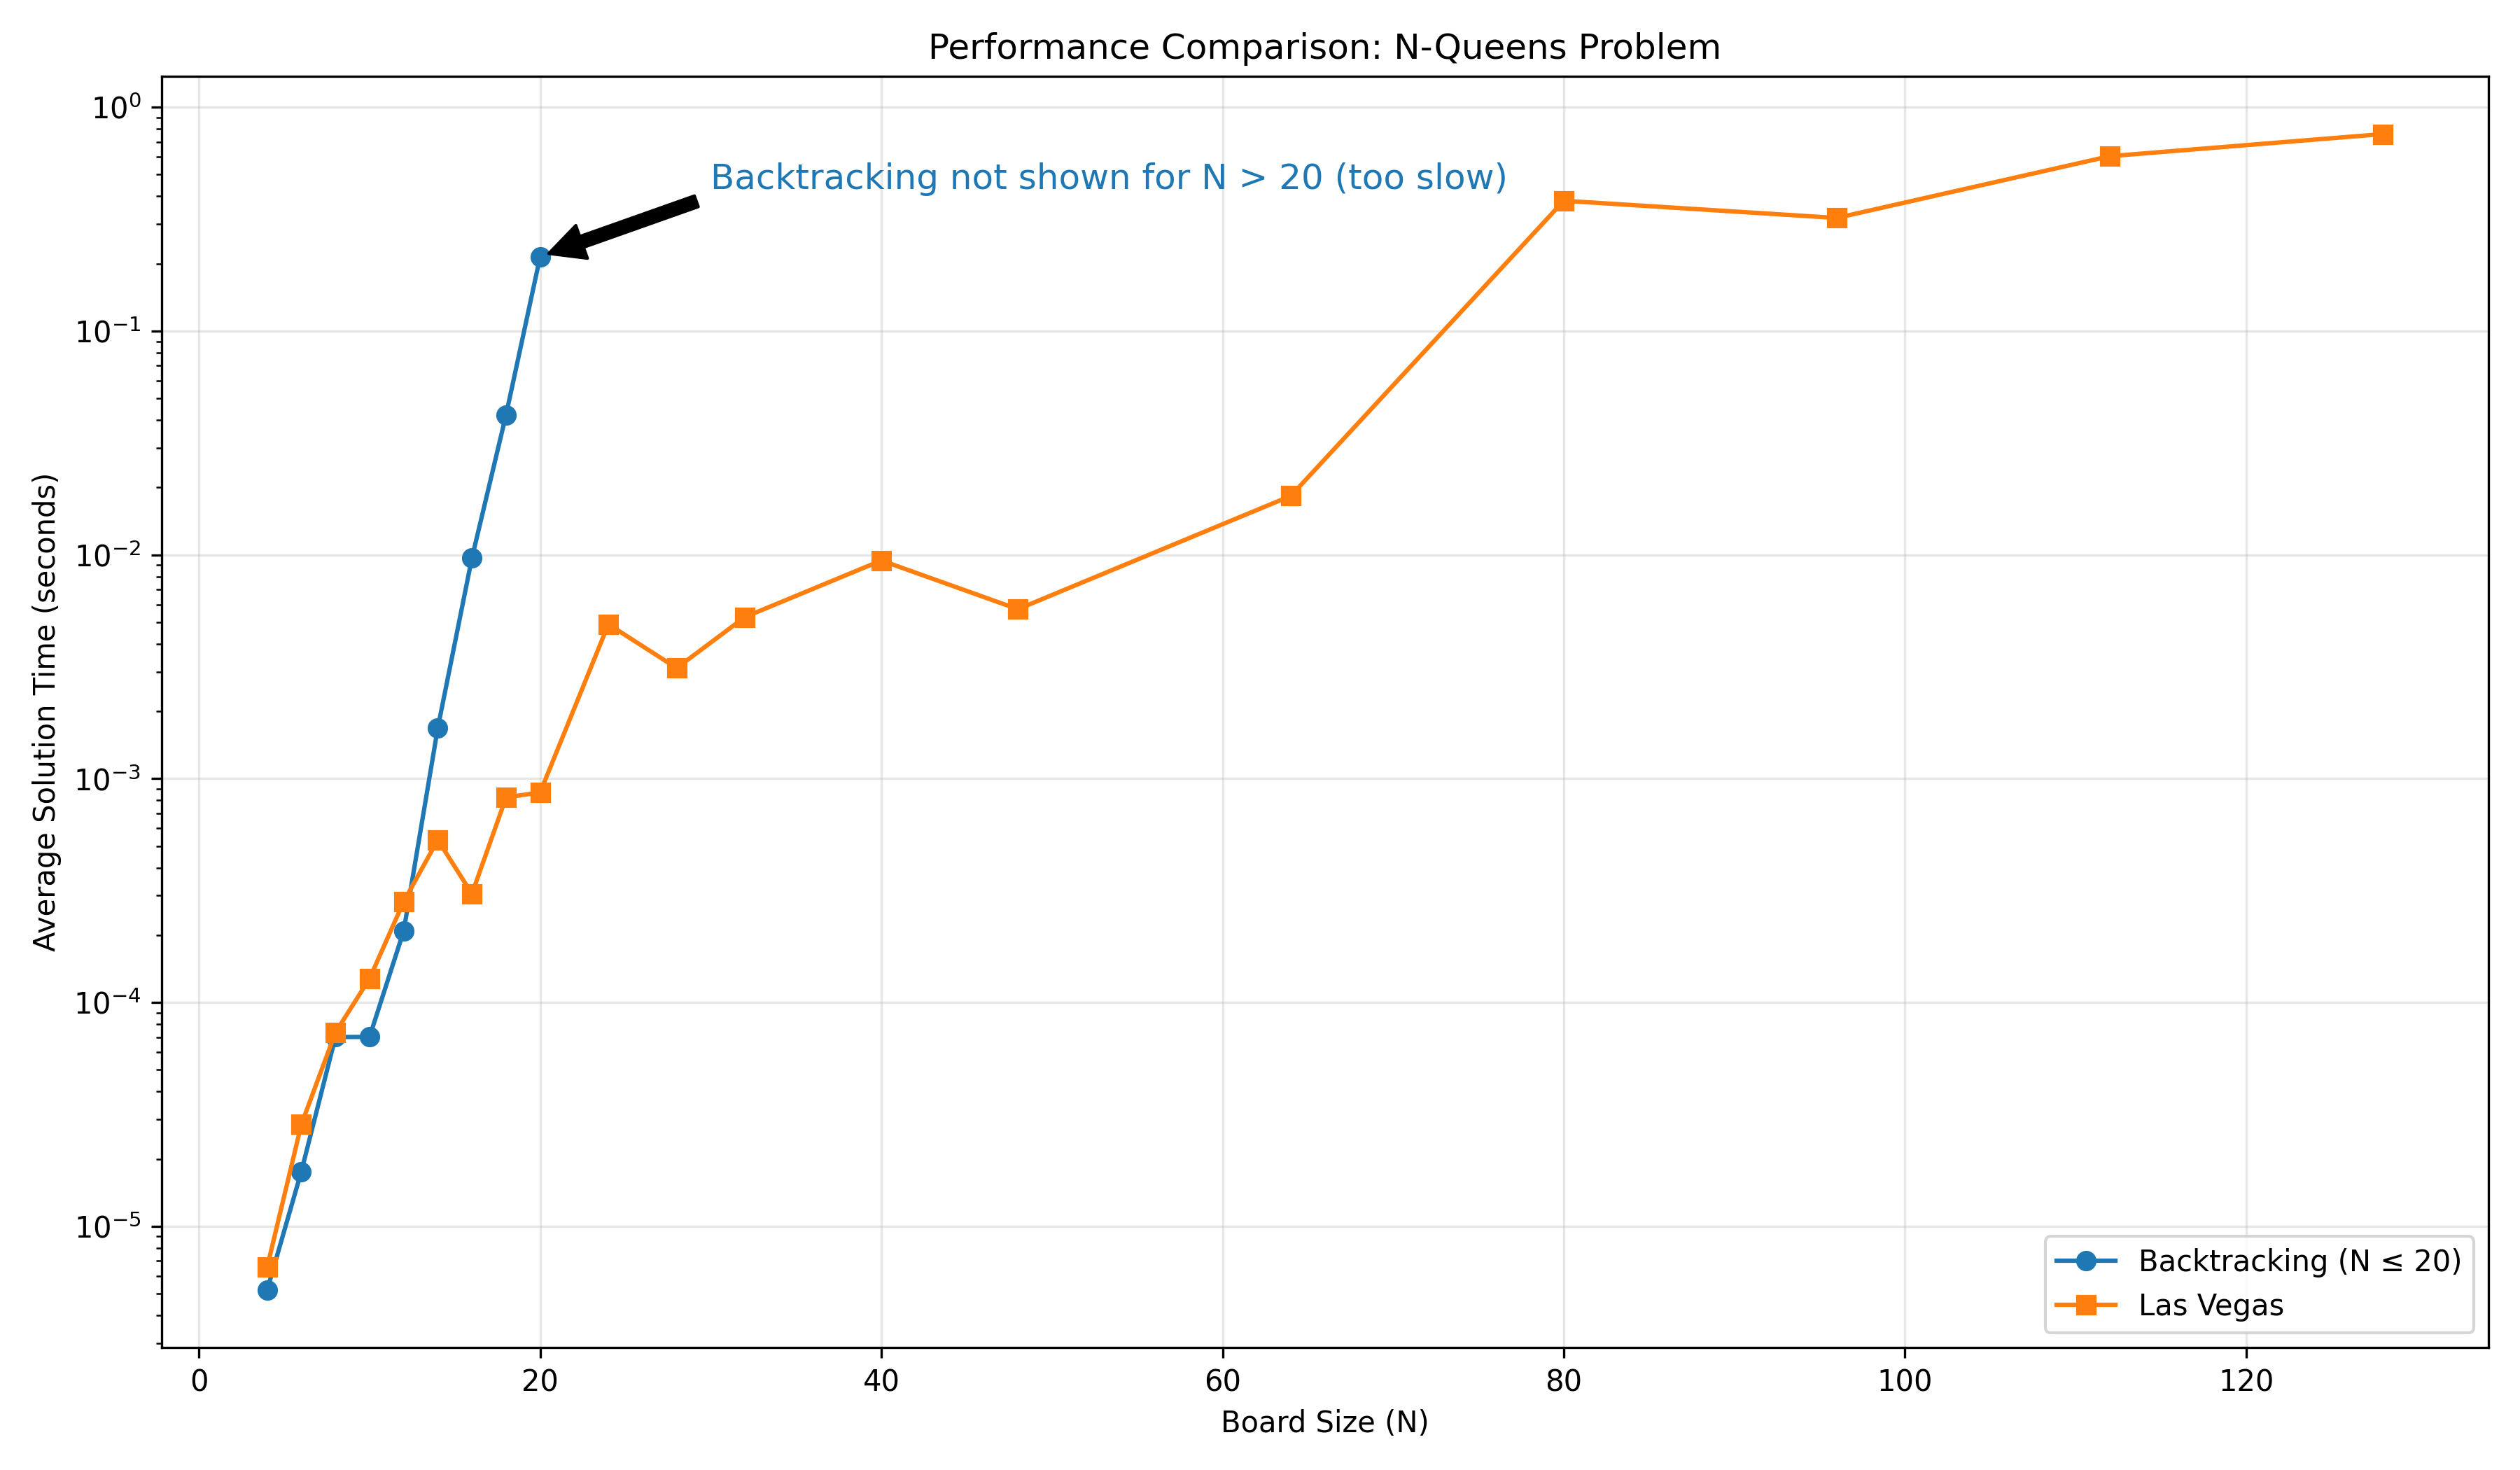
\includegraphics[height=0.95\textheight]{./programs/nqueens-lv/images/performance-comparison.png}
  \end{center}
  \vfill
\end{frame}

\begin{frame}{Performance Comparison (Interpretation)}
  \begin{itemize}
    \item Average solution time vs. $N$ for Backtracking and Las Vegas approaches.
    \item Las Vegas (randomized) is much faster for large $N$.
    \item Backtracking becomes infeasible as $N$ grows.
  \end{itemize}
\end{frame}

\begin{frame}{Performance Comparison}
  \begin{itemize}
    \item \textbf{Backtracking:}
          \begin{itemize}
            \item Deterministic, exhaustive search
            \item Predictable but slow for large $N$
          \end{itemize}
    \item \textbf{Las Vegas:}
          \begin{itemize}
            \item Randomized, may restart
            \item Runtime varies, but much faster on average for large $N$
          \end{itemize}
  \end{itemize}
\end{frame}

\begin{frame}{Key Insights}
  \begin{itemize}
    \item Randomization can dramatically improve performance for some combinatorial problems \parencite{motwani1995randomized}
    \item Las Vegas algorithms always produce correct results, but runtime is a random variable \parencite{lasvegas1979babai}
    \item For N-Queens, Las Vegas approach is practical for very large $N$ where backtracking is infeasible
    \item Illustrates the power of probabilistic algorithms in search and optimization
  \end{itemize}
\end{frame}

\begin{frame}{Monte Carlo Method - Estimating $\pi$}
  The Monte Carlo method estimates $\pi$ by simulating random points in a unit square and counting how many fall inside a quarter circle of radius 1. The ratio of points inside the circle to the total points, multiplied by 4, approximates $\pi$.
\end{frame}



\begin{frame}{Monte Carlo Algorithm}
  \begin{enumerate}
    \item Generate $N$ random points $(x, y)$ where $0 \leq x \leq 1$ and $0 \leq y \leq 1$.
    \item For each point, check if it lies inside the quarter circle: $x^2 + y^2 \leq 1$.
    \item Count the number of points $M$ that satisfy the condition.
    \item Estimate $\pi$ as: $\pi \approx 4 \times \frac{M}{N}$.
  \end{enumerate}
\end{frame}

\begin{frame}{Visual Illustration}
  \begin{center}
    \begin{tikzpicture}[scale=3.5]
      % Draw square and quarter circle
      \draw[thick] (0,0) rectangle (1,1);
      \draw[thin, blue] (0,1) arc (90:0:1);

      \foreach \i in {1,...,300} {
      \pgfmathsetmacro{\x}{rnd}
      \pgfmathsetmacro{\y}{rnd}
      \pgfmathsetmacro{\r}{\x*\x + \y*\y}

        \ifdim\r pt<1pt
          \fill[green!70!black] (\x,\y) circle (0.005);
        \else
          \fill[red!70!black] (\x,\y) circle (0.005);
        \fi
        }

      % Labels
      \node[anchor=north] at (0.5,0) {Unit Square};
      \node[blue, anchor=west] at (0.6,0.3) {Quarter Circle};
    \end{tikzpicture}
  \end{center}
\end{frame}


\begin{frame}{Example Calculation}
  \begin{itemize}
    \item Suppose we generate $N = 1000$ random points in the unit square
    \item After simulation, we count $M = 785$ points inside the quarter circle
    \item We estimate $\pi$ as:
          \[ \pi \approx 4 \times \frac{M}{N} = 4 \times \frac{785}{1000} = 3.14 \]
    \item The true value of $\pi$ is approximately $3.14159$
  \end{itemize}
\end{frame}

\begin{frame}{Convergence and Error Analysis}
  \begin{itemize}
    \item The error in our estimate decreases as $O(1/\sqrt{N})$
    \item This means:
          \begin{itemize}
            \item $N=100$ points gives roughly 10\% error
            \item $N=10,000$ points gives roughly 1\% error
            \item $N=1,000,000$ points gives roughly 0.1\% error
          \end{itemize}
    \item The Monte Carlo method is especially useful for calculating multidimensional integrals
    \item For $\pi$ calculation, there are more efficient methods, but this one is visually intuitive
  \end{itemize}
\end{frame}

\begin{frame}{Demo Visualization}
\begin{center}
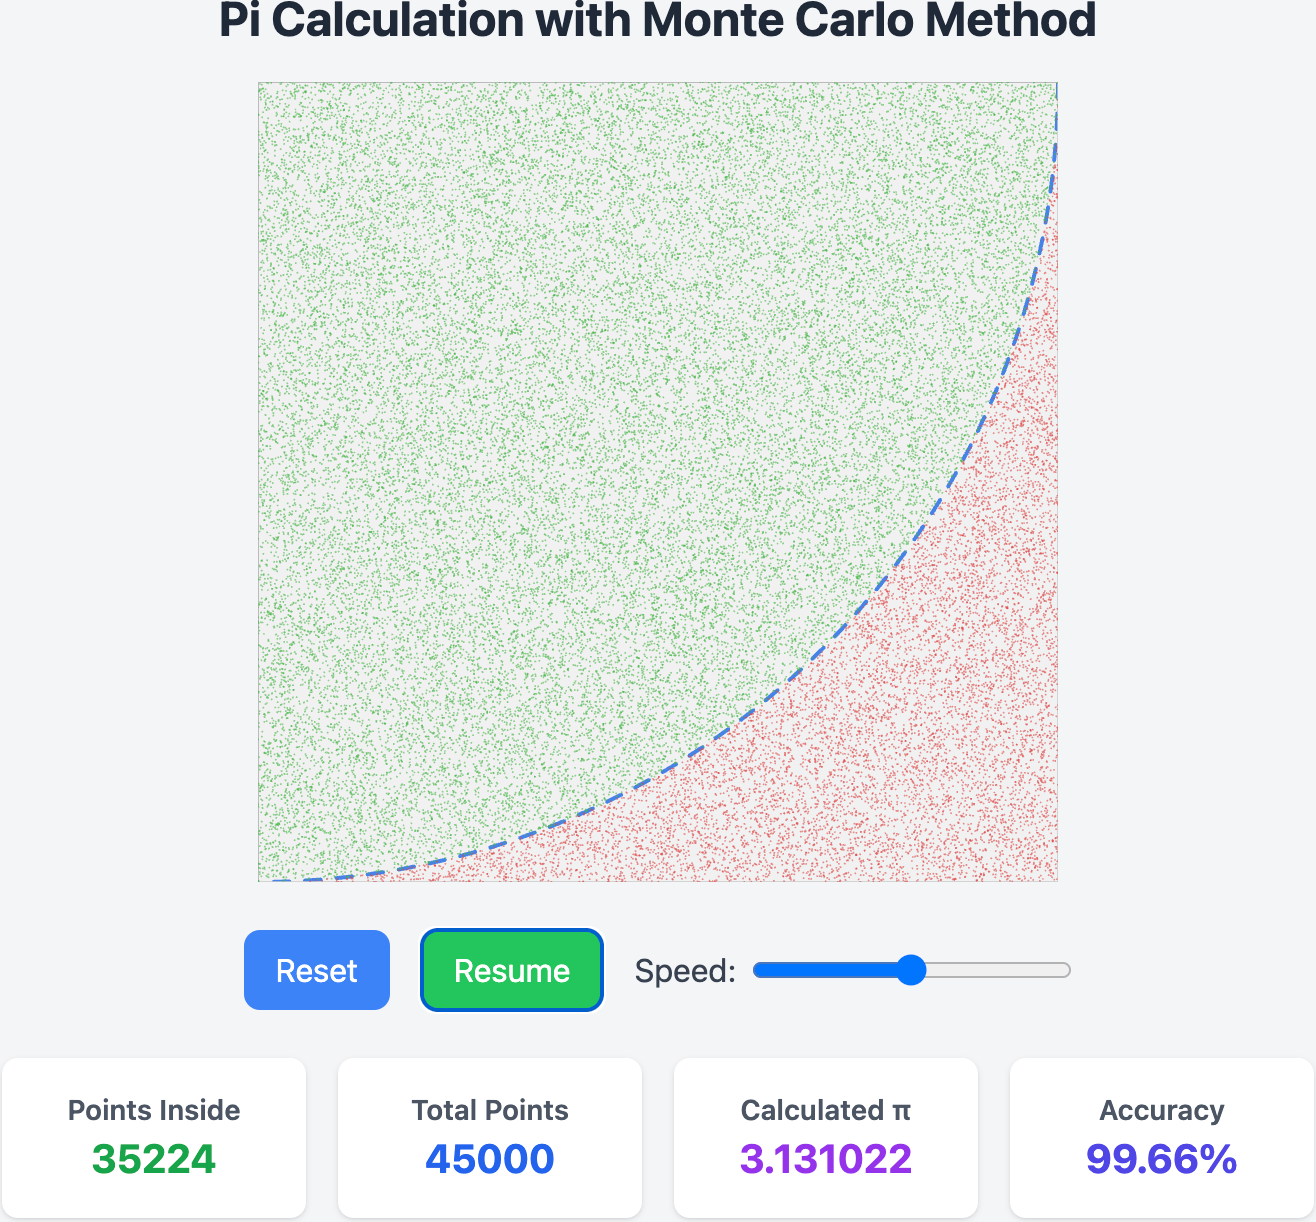
\includegraphics[width=0.4\textwidth]{../programs/pi_calculation/pi_calculation.png}

    \vspace{0.5cm}
    \href{../programs/pi_calculation/pi_calculation.html}{Open Interactive Demo}
    \end{center}
\end{frame}

% Probabilistic Data Structures
\section{Probabilistic Data Structures}
\begin{frame}{Deterministic vs. Probabilistic Data Structures}
  \begin{columns}
    \begin{column}{0.5\textwidth}
      \textbf{Deterministic (e.g., Hash Set, List):}
      \begin{itemize}
        \item Always provide exact answers.
        \item Can be space-intensive (store all elements).
        \item Operations might be slower for large datasets (e.g., disk I/O).
        \item \textbf{Guarantee:} No errors (false positives or negatives).
      \end{itemize}
    \end{column}
    \begin{column}{0.5\textwidth}
      \textbf{Probabilistic (e.g., Bloom Filter):}
      \begin{itemize}
        \item Provide approximate answers with controlled error.
        \item Very space-efficient (use bits, not full elements).
        \item Operations are typically very fast (constant time).
        \item \textbf{Trade-off:} Small error probability for huge efficiency gains.
      \end{itemize}
    \end{column}
  \end{columns}

  \begin{block}{Key Idea}
    Use PDS when approximate answers are acceptable and space/speed are critical.
  \end{block}
\end{frame}

\begin{frame}{Example: Why PDS? Username Availability}
  \begin{block}{The Problem}
    A website with millions of users needs to instantly check if a username is available during registration. How?
  \end{block}

  \begin{columns}
    \begin{column}{0.5\textwidth}
      \textbf{Deterministic Approach (Database Query):}
      \begin{itemize}
        \item Store all usernames in a database.
        \item Query DB: `SELECT 1 FROM users WHERE username = ?`
        \item \textbf{Accurate? Yes.}
        \item \textbf{Fast? No.} Requires disk I/O, network latency.
        \item \textbf{Scalable? Poorly.} High load on DB servers.
      \end{itemize}
    \end{column}
    \begin{column}{0.5\textwidth}
      \textbf{Probabilistic Approach (Bloom Filter):}
      \begin{itemize}
        \item Keep a compact Bloom filter in memory.
        \item Check filter: Is `username` possibly present?
        \item \textbf{Accurate? Mostly.} Small chance of false positive (saying taken when available), needs DB check then.
        \item \textbf{Fast? Yes.} In-memory check is O(k).
        \item \textbf{Scalable? Excellently.} Drastically reduces DB load.
      \end{itemize}
    \end{column}
  \end{columns}
\end{frame}

\begin{frame}{Username Checking: Implementation Details}
  \begin{enumerate}
    \item \textbf{Initialization:} Load all existing usernames into Bloom filter at service startup (only infrequent DB reads).
    \item \textbf{New registrations:} Add username to both database and Bloom filter.
    \item \textbf{Availability check process:}
          \begin{itemize}
            \item Check username against Bloom filter first (Fast, in-memory)
            \item If Bloom filter says "definitely not in set" $\rightarrow$ Username is available (99\% case for 1\% error rate)
            \item If Bloom filter says "possibly in set" $\rightarrow$ Verify with database query (Slow, but rare)
          \end{itemize}
  \end{enumerate}

  \begin{block}{Performance Impact (10M users, 1\% error)}
    \begin{itemize}
      \item Memory: $\approx 18$ MB Bloom Filter vs. hundreds of MB for DB index/cache.
      \item Speed: 99\% of availability checks avoid slow database queries.
    \end{itemize}
  \end{block}
\end{frame}


\begin{frame}{Username Checking: System Architecture}
  \begin{center}
    \begin{tikzpicture}[
        block/.style={rectangle, draw, text width=2cm, text centered, minimum height=1cm},
        line/.style={draw, -latex},
        cloud/.style={draw, ellipse, minimum width=2cm, minimum height=1cm}
      ]

      % Client and servers
      \node[block] (client) at (0,0) {Client};
      \node[block] (api) at (4,0) {API Server};
      \node[block] (bloom) at (8,1) {Bloom Filter (Memory)};
      \node[block] (db) at (8,-1) {Database (Disk)};

      % Connections
      \path[line] (client) -- node[above] {Check username} (api);
      \path[line] (api) -- node[above] {1. Check Filter} (bloom);
      \path[line] (api) -- node[below] {2. Verify if needed} (db);

      % Fast path annotation
      \draw[dashed, thick, green!60!black, ->] (bloom) to[out=135, in=45] node[above] {Fast 'Available' (99\%)} (api);

      % Load path
      \path[line, gray] (db) -- node[right] {Initial load} (bloom);
    \end{tikzpicture}
  \end{center}

  \begin{itemize}
    \item Bloom filter acts as a fast, efficient preliminary check.
    \item Deterministic check (DB) used only as a fallback.
    \item Massively reduces load on the expensive resource (Database).
  \end{itemize}
\end{frame}

\begin{frame}{Bloom Filters: The Theory}
  \begin{columns}
    \begin{column}{0.6\textwidth}
      \begin{itemize}
        \item Space-efficient probabilistic data structure
        \item Tests if an element is a member of a set
        \item Possible false positives, never false negatives
        \item Components:
              \begin{itemize}
                \item Bit array of $m$ bits (initially all 0)
                \item $k$ independent hash functions
              \end{itemize}
      \end{itemize}
    \end{column}
    \begin{column}{0.4\textwidth}
      \begin{tikzpicture}[scale=0.5]
        % Draw bit array
        \foreach \i in {0,...,7} {
            \draw (\i,0) rectangle (\i+1,1);
            \node at (\i+0.5,0.5) {0};
          }

        % Show set bits
        \node at (1.5,0.5) {\textcolor{red}{1}};
        \node at (4.5,0.5) {\textcolor{red}{1}};
        \node at (6.5,0.5) {\textcolor{red}{1}};
      \end{tikzpicture}
    \end{column}
  \end{columns}
\end{frame}

\begin{frame}{Bloom Filter Operations}
  \begin{columns}
    \begin{column}{0.5\textwidth}
      \textbf{Add element:}
      \begin{enumerate}
        \item Hash element with $k$ functions
        \item Set bits at these $k$ positions to 1
      \end{enumerate}

      \textbf{Query element:}
      \begin{enumerate}
        \item Hash element with $k$ functions
        \item Check bits at these $k$ positions
        \item If \textbf{any} bit is 0: \textcolor{red}{Definitely not in set}
        \item If \textbf{all} bits are 1: \textcolor{orange}{Probably in set}
      \end{enumerate}
    \end{column}
    \begin{column}{0.5\textwidth}
      \begin{tikzpicture}[scale=0.5]
        % Draw bit array
        \foreach \i in {0,...,7} {
            \draw (\i,0) rectangle (\i+1,1);
            \node at (\i+0.5,0.5) {0};
          }

        % Update for apple
        \node at (1.5,0.5) {\textcolor{red}{1}};
        \node at (4.5,0.5) {\textcolor{red}{1}};
        \node at (6.5,0.5) {\textcolor{red}{1}};

        % Draw element and hash functions
        \node at (4,-1.5) {Query: "apple"};
        \draw[->] (4,-1.2) -- (1.5,0);
        \draw[->] (4,-1.2) -- (4.5,0);
        \draw[->] (4,-1.2) -- (6.5,0);
      \end{tikzpicture}
    \end{column}
  \end{columns}
\end{frame}

\begin{frame}{The Math Behind Bloom Filters}
  \begin{itemize}
    \item \textbf{False positive probability ($p$):}
          \begin{equation}
            p \approx \left(1 - e^{-kn/m}\right)^k
          \end{equation}

    \item \textbf{Optimal size ($m$ bits) for $n$ items, error $p$:}
          \begin{equation}
            m = -\frac{n \ln p}{(\ln 2)^2}
          \end{equation}

    \item \textbf{Optimal hash functions ($k$):}
          \begin{equation}
            k = \frac{m}{n} \ln 2 \approx 0.7 \cdot \frac{m}{n}
          \end{equation}
  \end{itemize}
\end{frame}

\begin{frame}{Time and Space Complexity}
  \begin{center}
    \begin{tabular}{l|c|c|c|c}
      \textbf{Structure} & \textbf{Space} & \textbf{Lookup} & \textbf{Insert} & \textbf{Error Type} \\
      \hline
      Hash Set           & $O(n)$         & $O(1)$ avg      & $O(1)$ avg      & None                \\
      Bloom Filter       & $O(m)$         & $O(k)$          & $O(k)$          & False Positives     \\
      Sorted List        & $O(n)$         & $O(\log n)$     & $O(n)$          & None                \\
      Trie               & $O(N)$         & $O(L)$          & $O(L)$          & None                \\
    \end{tabular}
  \end{center}

  $n$=items, $m$=bits ($m \ll n \times item\_size$), $k$=hashes, $N$=total chars, $L$=key length
\end{frame}

\begin{frame}{Other Applications of Bloom Filters}
  \vspace{0.5cm}
  \begin{columns}
    \begin{column}{0.5\textwidth}
      \textbf{Web/Database:}
      \begin{itemize}
        \item Cache hit/miss optimization (e.g., CDNs)
        \item Avoid unnecessary DB lookups (like username example)
        \item Recommendation systems (seen items)
      \end{itemize}
      \pause

      \textbf{Network:}
      \begin{itemize}
        \item Web crawler URL deduplication (avoid re-crawling)
        \item Network packet routing (track flows efficiently)
        \item P2P network resource discovery
      \end{itemize}
      \pause
    \end{column}
    \begin{column}{0.5\textwidth}
      \textbf{Security:}
      \begin{itemize}
        \item Malware signature detection
        \item Spam filtering (known bad IPs/domains)
        \item Password breach checking (HaveIBeenPwned)
      \end{itemize}
      \pause

      \textbf{Big Data:}
      \begin{itemize}
        \item Stream deduplication (unique visitors/events)
        \item Distributed data sync (approximate differences)
        \item Genomics (k-mer counting)
      \end{itemize}
      \pause
    \end{column}
  \end{columns}
\end{frame}

\begin{frame}{When to Use Bloom Filters}
  Bloom filters are ideal when:

  \begin{itemize}
    \item Memory is a critical constraint (Big Data, embedded systems)
    \item False positives are acceptable (can be handled by a secondary check)
    \item False negatives are unacceptable (must find all true positives)
    \item Elements are expensive to store or compare
    \item Lookup speed is crucial (real-time systems)
    \item Deletions are not needed (or use variants like Counting Bloom Filters)
  \end{itemize}
\end{frame}


\begin{frame}[allowframebreaks]
  \printbibliography
\end{frame}

\end{document}
